
%\UseRawInputEncoding
\documentclass{article}
\setcounter{secnumdepth}{0}
\usepackage[T1]{fontenc}
\usepackage[utf8]{inputenc}
%\usepackage[latin1]{inputenc}
%\usepackage[english, norsk]{babel}
\usepackage{filecontents}
\usepackage{tcolorbox}
\usepackage{url}
\usepackage{etoolbox}
\usepackage{framed}
\usepackage{framed, color}
\usepackage{xcolor}
\usepackage{mdframed}
\usepackage{float}
\usepackage{gensymb}
\usepackage{amsmath}

\definecolor{Black}{rgb}{0.0, 0.0, 0.0}

%Definer kode
\usepackage{listings}
\usepackage{color}
\definecolor{dkgreen}{rgb}{0,0.6,0}
\definecolor{gray}{rgb}{0.5,0.5,0.5}
\definecolor{mauve}{rgb}{0.58,0,0.82}

\lstset{frame=tb,
extendedchars = true,
texcl=true,
  language=C++,
  aboveskip=3mm,
  belowskip=3mm,
  showstringspaces=false,
  columns=flexible,
  basicstyle={\small\ttfamily},
  numbers=none,
  numberstyle=\tiny\color{gray},
  keywordstyle=\color{blue},
  commentstyle=\color{dkgreen},
  stringstyle=\color{mauve},
  breaklines=true,
  breakatwhitespace=true,
  tabsize=3
}

\usepackage[colorlinks]{hyperref}
\hypersetup{citecolor=Black}
\hypersetup{linkcolor=Black}
\hypersetup{urlcolor=Black}
\usepackage{cleveref}


\setlength{\parindent}{0em}
\setlength{\parskip}{1em}
%\renewcommand{\baselinestretch}{2.0}

%\renewcommand\thesubsection{\alph{subsection}}

\renewcommand{\figurename}{Figure}
\begin{document}
\author{Kent Odde}
\title{DCS3101\\Assignment 3}

\maketitle
\thispagestyle{empty}
\begin{center}
\includegraphics[width=\linewidth,height=0.2\textheight,keepaspectratio]{img/USN.png}
\end{center}
\newpage

\tableofcontents

\newpage

\section{Abstract}

This is my submission for the third compulsory assignment in DCS3101, Introduction to Cybersecurity.




\section{Q1}
\begin{tcolorbox}\textit{What are the advantages of firewalls?}\end{tcolorbox}
A firewall is a component, that functions as a check-point in a network, and its job is to monitor and regulate traffic passing through it.

The main use case and advantage of a firewall, is that we can protect a local trusted network against threats which might exist on another untrusted network.

When implemented, all traffic passing from network A to network B must pass through the firewall. The firewall may prohibit traffic it considers a threat. This decision has traditionally been based on a predefined ruleset, but next-generation firewalls have much more sophisticated methods of identifying potential threats.

A strength of firewalls is their wide range of types suitable for different needs, and their capability for configuration. We can have an open firewall, where we define rules for what the firewall should filter out, or for a more conservative approach, we can have a firewall which filters all packages, and we whitelist the traffic we do want.

We can filter traffic based the sender or receiver or by the contents of the packets, which can be used to protect specific hosts or specific ports. We can filter based on the types of application layer protocol the package contains, which can help us filter out spam mail etc. We can also use the TCP headers, so that an outgoing TCP packet on a port, will temporarily open the port for incoming packets, given that the TCP header contain the correct information.

There are also \textit{next-generation} firewalls, which can employ machine learning to be able to recognize unknown types of malicous traffic based on patterns.

As an added bonus of all this, we can also configure firewalls to log all traffic, which may be very handy for several reasons, but especially if we find out that our network has been compromised.


\newpage
\section{Q2}
\begin{tcolorbox}
  \textit{Comment if the following is true or false in the context of TLS - "The algorithms inside a session are negotiated between client and server." Justify your answer with an associated protocol diagram.}
\end{tcolorbox}
The statement in the question is \textbf{true}. Different clients and servers will have support for different encryption and MAC algorithms. Just like different people speak different languages. The goal of the negotiation is to find mutually supported algorithms, that are also recognized as secure enough by the current version of TLS.

However, negotiation is perhaps a strong word. If we look at subset of the TLS handshake protocol in figure \ref{TLS}, we can see that the client starts the conversation with a \textit{hello}.


\begin{figure}[H]
 \centering
  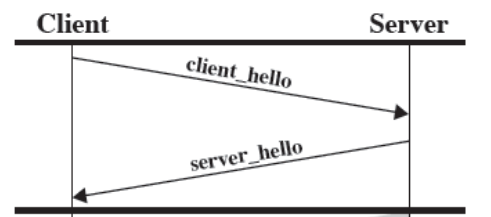
\includegraphics[width=200pt]{img/tlsHandshake.png}
 \caption{Part of the TLS handshake protocol diagram from lecture}
  \label{TLS}
 \end{figure}


This hello consists of information about the client, like what algorithms it has support for. One of the things the server then does, is to pick the strongest of these algorithms that it self supports. The server hello will then among other things, contain this decision.



\newpage
\section{Q3}
\begin{tcolorbox}
  \textit{It was discussed in the class about one particular attack on TLS. Discuss this attack and identify another attack that can impact TLS. Discuss briefly about the attack you have chosen for your answer.}
\end{tcolorbox}
The attack discussed in class was the exploitation of what has come to be known as the \textit{heartbleed bug}. This was a bug in the heartbeat protocol of TLS.

The heartbeat protocol, is a mechanism for letting the client check that the connection with the server is still active. The client would send a message asking for a distinct string as a reply, and the character length of this string. If the connection was still alive, the server would naturally send the requested string back.

However, it was discoverd that if the number containing the length of the string was much higher than the actual length of the string, the server would in addition to the string send random content of its RAM. This was of course catastrophic, as a web-servers RAM is filled with a lot of information that can be exploited, like encryption keys and so on.





\newpage
\section{Q4}
\begin{tcolorbox}
  \textit{What are the differences between IDS and IPS? Discuss on classification/taxonomy of IDS and IPS.}
\end{tcolorbox}





\section{Q5}
\begin{tcolorbox}
  \textit{Biometrics - What are the key factors for choosing a biometric modality (e.g., face, fingerprint, iris, etc)?}
\end{tcolorbox}


\section{Q6}
\begin{tcolorbox}
  \textit{What kind of attacks are possible on face biometric systems?}
\end{tcolorbox}










%Vedlegg
\section{Appendices}


\newpage
%Referanse
%\section{Referanser}

\nocite{*}
\bibliographystyle{plain}
\bibliography{ref}

\addcontentsline{toc}{section}{References}

\end{document}
